\documentclass{beamer}

% packages
\usepackage{multicol}
\usepackage[T2A]{fontenc}
\usepackage[utf8]{inputenc}
\usepackage[english,russian]{babel}
\usepackage{booktabs}
\usepackage{biblatex}
\usepackage{graphicx}
\usepackage{href-ul}
\usepackage{cmap}
\usepackage{svg}

\usepackage{lipsum}

% math packages
\usepackage{amsmath,amsfonts,amssymb,amsthm,mathtools}
\usepackage{mathtext}
\usepackage{icomma}
\usepackage{floatflt}

% settings
\setbeamertemplate{navigation symbols}{}
\setbeamertemplate{section in toc}[sections numbered]
\setlength{\columnseprule}{0.2pt}

%%%%%%%%%%%%%%%%%%%%%%%%%%%%%%%%%%
% Metropolis Theme Configuration %
%%%%%%%%%%%%%%%%%%%%%%%%%%%%%%%%%%

\usetheme[
    %%% main theme %%%
    titleformat=regular, 
    %%% inner theme %%%
    sectionpage=progressbar, % + slide
    %sectionpage=none, % disables section page
    %%% outer theme %%%
    numbering=fraction,
    progressbar=frametitle,
    %%% color theme %%%
    block=transparent,
    background=light
]{metropolis}

%%%%%%%%%%%%% Title %%%%%%%%%%%%%%

\setbeamertemplate{title page}{
  \begin{minipage}[b][\paperheight]{\textwidth}
    \centering  % <-- Center here
    \ifx\inserttitlegraphic\@empty\else\usebeamertemplate*{title graphic}\fi
    \vfill%
    \ifx\inserttitle\@empty\else\usebeamertemplate*{title}\fi
    \ifx\insertsubtitle\@empty\else\usebeamertemplate*{subtitle}\fi
    \usebeamertemplate*{title separator}
    \ifx\beamer@shortauthor\@empty\else\usebeamertemplate*{author}\fi
    \ifx\insertinstitute\@empty\else\usebeamertemplate*{institute}\fi
    \vspace*{0.5cm}
    \ifx\insertdate\@empty\else\usebeamertemplate*{date}\fi
    \vfill
    \vspace*{1mm}
  \end{minipage}
}

\setbeamertemplate{title}{
%  \raggedright%  % <-- Comment here
  \linespread{1.0}%
  \inserttitle%
  \par%
  \vspace*{0.5em}
}
\setbeamertemplate{subtitle}{
%  \raggedright%  % <-- Comment here
  \insertsubtitle%
  \par%
  \vspace*{0.5em}
}

%%%%%%%%%%%%% Blocks %%%%%%%%%%%%%

% map defaulf block to oldblock
\let\oldblock\block
\let\endoldblock\endblock

% change block by adding smallskip
\renewenvironment{block}[1]
{\begin{oldblock}{#1}
    \smallskip
}
{ 
\end{oldblock}
}

\setbeamerfont{bibliography entry title}{size=}
\setbeamerfont{bibliography entry author}{size=}
\setbeamerfont{bibliography entry location}{size=}
\setbeamerfont{bibliography entry note}{size=}

%%%%%%%%%%%%% Colors %%%%%%%%%%%%%

\setbeamercolor{normal text}{fg=black, bg=white}
\setbeamercolor{progress bar}{fg=normal text.fg, bg=normal text.fg!50!black!30} 
\setbeamercolor{frametitle}{fg=normal text.fg, bg=normal text.bg}
\createthesistitle

\begin{document}

%=======
\begin{frame}[noframenumbering,plain]
	%\thispagestyle{empty}
	\titlepage
\end{frame}
%=======
\begin{frame}{Байесовский выбор достаточного размера выборки}
    Исследуется задача выбора достаточного размера выборки.
    \vfill
    \begin{block}{Проблема}
        Большинство подходов используют распределение параметров модели. Статистические методы требуют для оценки избыточный размер доступной выборки.
    \end{block}
    \vfill
    \begin{block}{Цель}
        Требуется предложить метод, не использующий напрямую параметры модели. Необходимо учесть недостаточный размер доступной выборки.
    \end{block}
    \vfill
    \begin{block}{Решение}
        Предлагается использовать функцию правдоподобия выборки. Рассматривается подход в случаях избыточного и недостаточного размеров доступной выборки. 
    \end{block}
\end{frame}
%=======
\begin{frame}{Постановка задачи выбора размера выборки}
    \begin{block}{Выборка}
        \vspace{-0.3cm}
        \[ \mathfrak{D}_m = \left\{ \bx_i, y_i \right\}_{i = 1}^{m}, \ \bx_i \in \mathbb{X}, \ y_i \in \mathbb{Y}. \]
        \vspace{-0.7cm}
    \end{block}
    \begin{block}{Параметризация распределения}
        \vspace{-0.3cm}
        \[ p(y | \bx) \quad \longrightarrow \quad p(y | \bx, \bw), \ \bw \in \mathbb{W}. \]
        \vspace{-0.7cm}
    \end{block}
    \begin{block}{Функция правдоподобия выборки}
        \vspace{-0.5cm}
        \[ L(\mathfrak{D}_m, \bw) = \prod_{i=1}^{m} p(y_i | \bx_i, \bw), \qquad l(\mathfrak{D}_m, \bw) = \sum\limits_{i=1}^{m} \log p(y_i | \bx_i, \bw). \]
        \vspace{-0.5cm}
    \end{block}
    \begin{block}{Оценка максимального правдоподобия}
        \vspace{-0.3cm}
        \[ \hat{\bw}_{m} = \arg\max_{\bw} L(\mathfrak{D}_m, \bw). \]
        \vspace{-0.7cm}
    \end{block}
    \begin{block}{Цель}
        Требуется определить достаточный размер выборки $m^*$.
    \end{block}
\end{frame}
%=======
\begin{frame}{Достаточный размер выборки не превосходит доступный}
    Рассмотрим выборку $\mathfrak{D}_k$ размера $k \leqslant m$. Оценим на ней параметры, используя метод максимума правдоподобия:
    \[ \hat{\mathbf{w}}_{k} = \arg\max_{\mathbf{w}} L(\mathfrak{D}_k, \mathbf{w}). \]
    Зафиксируем некоторое положительное число $\varepsilon > 0$.
    \begin{rusdefinition}[D-достаточный размер выборки]
        Размер выборки $m^*$ называется \textbf{D-достаточным}, если для любого $k \geqslant m^*$
        \[ D(k) = \mathbb{D}_{\mathfrak{D}_k} L(\mathfrak{D}_m, \hat{\mathbf{w}}_{k}) \leqslant \varepsilon. \]
    \end{rusdefinition}
    \begin{rusdefinition}[M-достаточный размер выборки]
        Размер выборки $m^*$ называется \textbf{M-достаточным}, если для любого $k \geqslant m^*$ 
        \[ M(k) = \left| \mathbb{E}_{\mathfrak{D}_{k+1}} L(\mathfrak{D}_m, \hat{\mathbf{w}}_{k+1}) - \mathbb{E}_{\mathfrak{D}_k} L(\mathfrak{D}_m, \hat{\mathbf{w}}_{k}) \right| \leqslant \varepsilon. \]
    \end{rusdefinition}
\end{frame}
%=======
\begin{frame}{Корректность M-определения}
    \begin{block}{Утверждение 1 (асимптотическая нормальность)}
        Пусть $\hat{\bw}_k$~--- оценка максимума правдоподобия $\bw$. Тогда при определенных условиях регулярности имеет место следующая сходимость по распределению:
        \[ \hat{\bw}_k \xrightarrow{d} \mathcal{N}\left(\bw, \left[m\mathcal{I}(\bw)\right]^{-1}\right). \]
    \end{block}
    \begin{alertblock}{Лемма 1}
        Пусть $\| \bm_k - \bw \|_2 \to 0$ и $\| \bSigma_k - \left[m\mathcal{I}(\bw)\right]^{-1} \|_{F} \to 0$ при $k \to \infty$. Тогда в модели линейной регрессии определение M-достаточного размера выборки является корректным. А именно, найдется такой $m^*$, что для всех $k \geqslant m^*$ выполнено $M(k) \leqslant \varepsilon$.
    \end{alertblock}
\end{frame}
%=======
\begin{frame}{Достаточный размер выборки больше доступного}
    \begin{block}{}
        Возникает задача прогнозирования математического ожидания и функции правдоподобия при $k > m$.
    \end{block}
    \begin{figure}[h!]
        \centering
        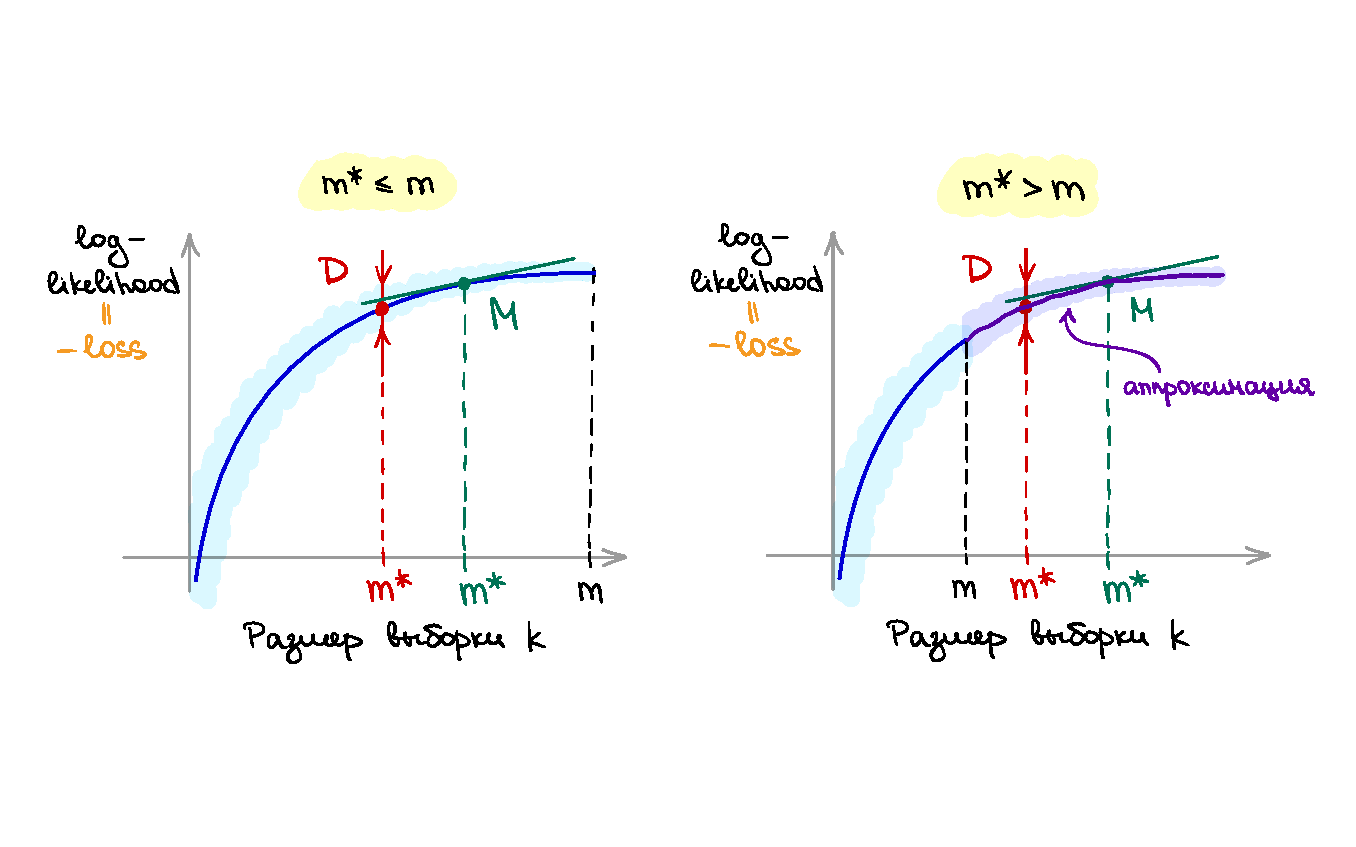
\includegraphics[width=\textwidth]{paper/figures/image.pdf}
        \label{image}
    \end{figure}
\end{frame}
%=======
\begin{frame}{Синтетическая выборка при $m^* \leqslant m$}
    \begin{center}
        Линейная регрессия
    \end{center}
    \begin{figure}[h!]
        \centering
        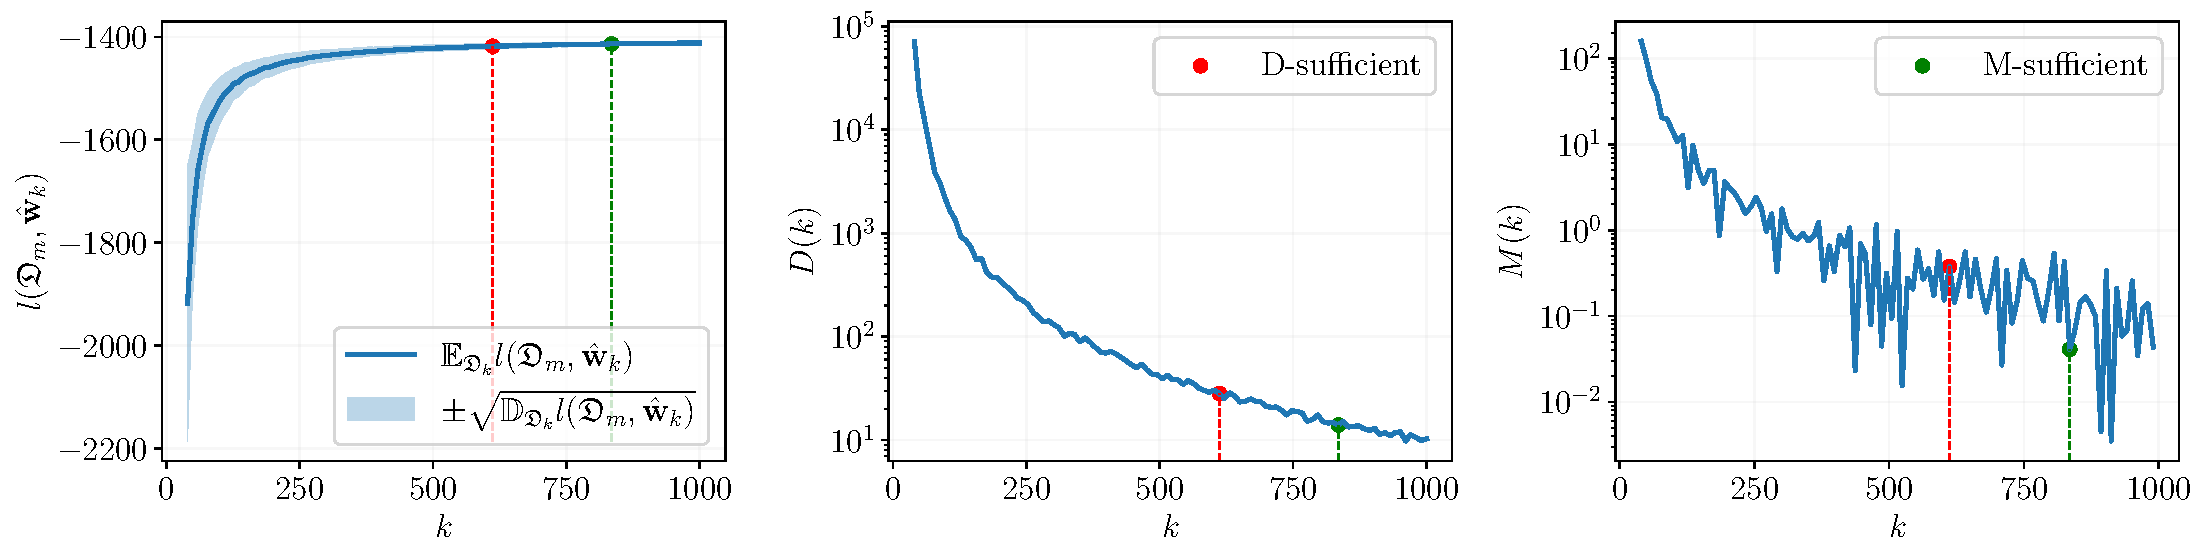
\includegraphics[width=\textwidth]{paper/figures/synthetic-regression-sufficient.pdf}
        \label{synthetic-regression-sufficient}
    \end{figure}
    \vspace{-1cm}
    \begin{center}
        Логистическая регрессия
    \end{center}
    \begin{figure}[h!]
        \centering
        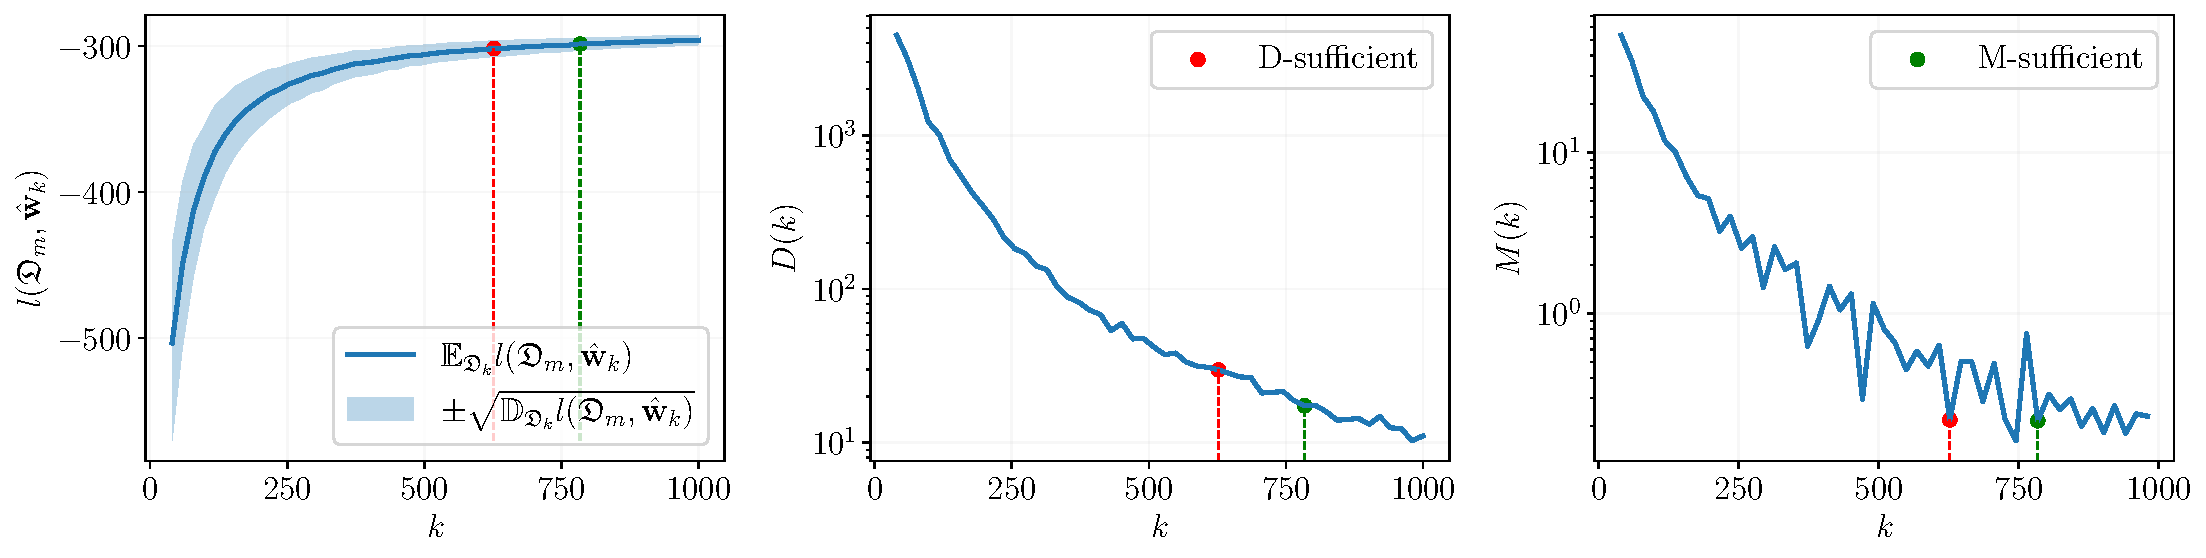
\includegraphics[width=\textwidth]{paper/figures/synthetic-classification-sufficient.pdf}
        \label{synthetic-classification-sufficient}
    \end{figure}
\end{frame}
%=======
\begin{frame}{Синтетическая выборка при $m^* > m$}
    Для синтетических выборок проведена аппроксимация функций правдоподобия. Среднее значение и дисперсия аппроксимированы соответственно функциями
    \[ \varphi(m) = a_1 - a_2^2 \exp\left( - a_3^2 m \right) - \dfrac{a_4^2}{m^{3/2}} \]
    и
    \[ \psi(m) = b_1^2 \exp\left( - b_2^2 m \right) + \dfrac{b_3^2}{m^{3/2}}, \]
    где $\mathbf{a}$ и $\mathbf{b}$~--- вектора параметров.
\end{frame}
%=======
\begin{frame}{Синтетическая выборка при $m^* > m$}
    \begin{center}
        Линейная регрессия
    \end{center}
    \begin{figure}[h!]
        \centering
        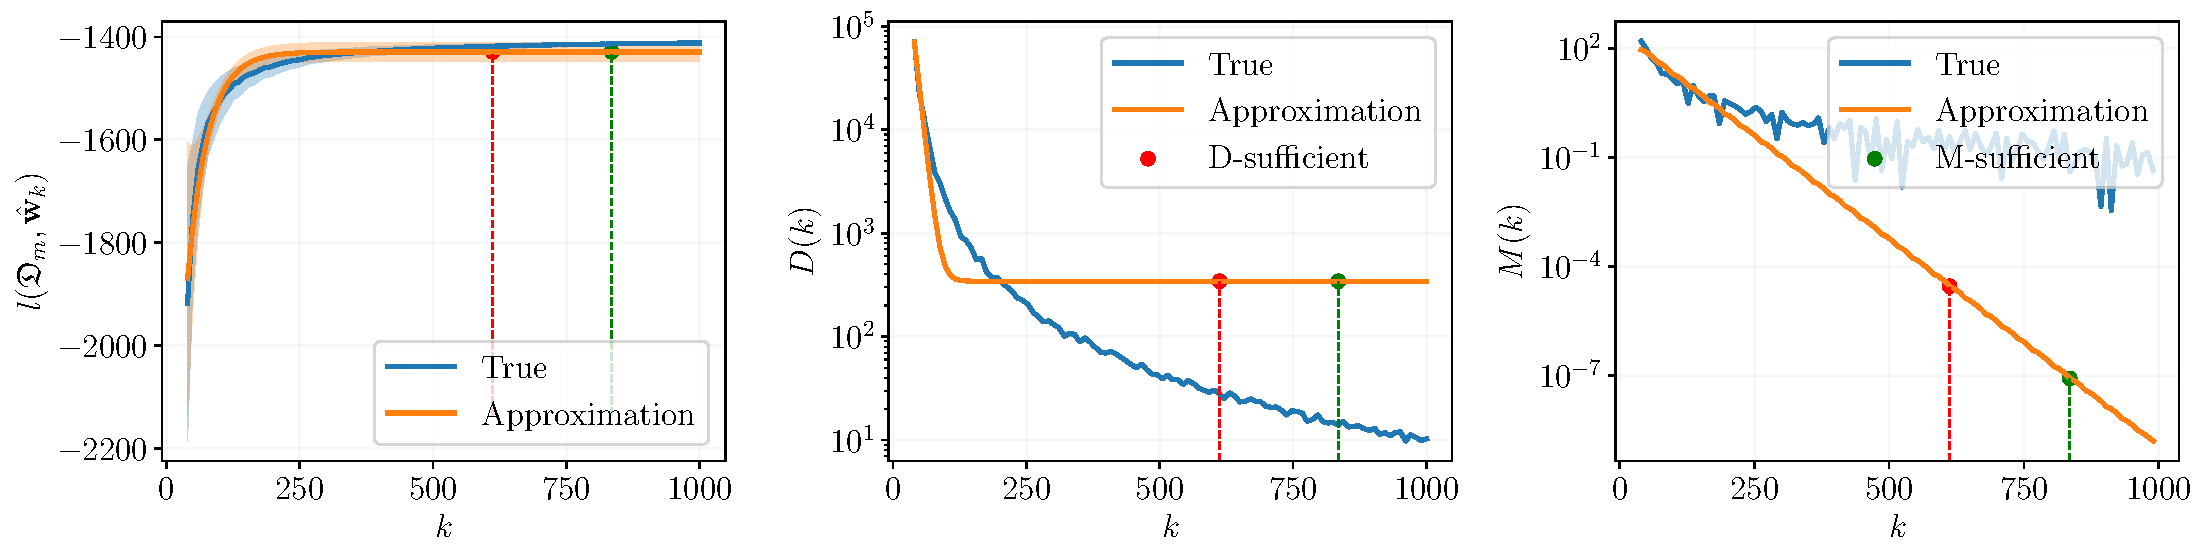
\includegraphics[width=\textwidth]{paper/figures/synthetic-regression-approximation.pdf}
        \label{synthetic-regression-approximation}
    \end{figure}
    \vspace{-1cm}
    \begin{center}
        Логистическая регрессия
    \end{center}
    \begin{figure}[h!]
        \centering
        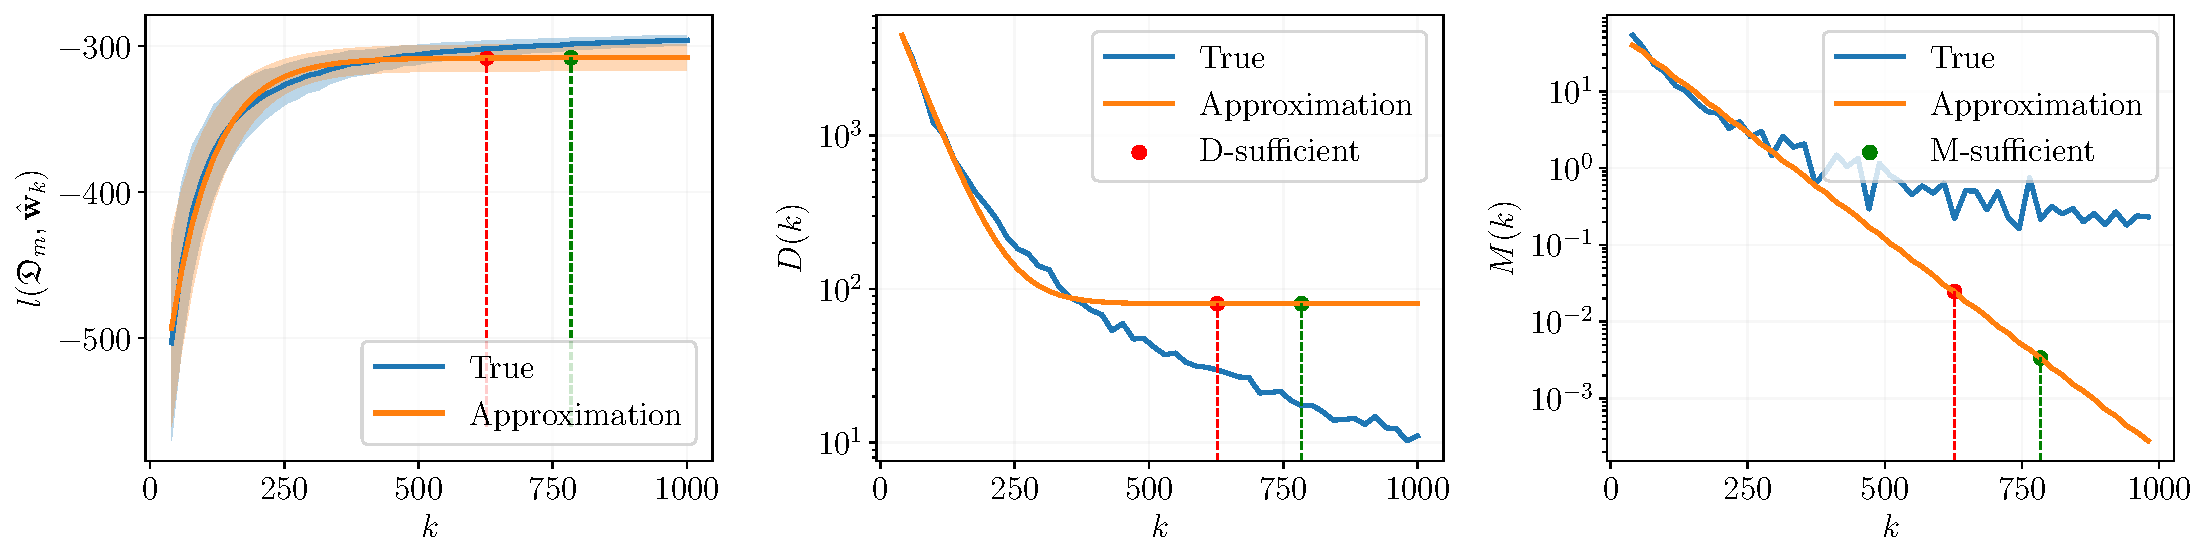
\includegraphics[width=\textwidth]{paper/figures/synthetic-classification-approximation.pdf}
        \label{synthetic-classification-approximation}
    \end{figure}
\end{frame}
%=======
\begin{frame}{Дальнейшие цели}
    \begin{itemize}
        \item Доказать корректность предложенных определений.
        \item Доказать <<хорошие>> свойства бутстрап-оценок математического ожидания и дисперсии функции правдоподобия выборки.
        \item Улучшить подход к прогнозированию функции правдоподобия при $m^* > m$.
    \end{itemize}
\end{frame}
%=======
%\begin{frame}{Выносится на защиту}
%    \begin{enumerate}
%        \item Это первое...
%        \vfill
%        \item Это второе...
%        \vfill
%        \item Это третье...
%    \end{enumerate}
%\end{frame}
%=======

\end{document} 